\documentclass[
  11pt,
  letterpaper,
   addpoints,
   answers
  ]{exam}

\usepackage{../exercise-preamble}

\begin{document}

\noindent
\begin{minipage}{0.47\textwidth}

\includegraphics[width=\textwidth]{../fcfm_die}
\end{minipage}
\begin{minipage}{0.53\textwidth}
\begin{center} 
\large\textbf{Fundamentos de control de sistemas} (EL4111-1) \\
\large\textbf{Clase auxiliar 1} \\
\small Prof.~Roberto Cardenas Dobson\\
\small Prof.~Aux.~Osvaldo Jimenez - Erik Sáez\\
\small Ayudantes.~Simon Arenas- Juan Pablo Baez - Francisco Garces - Sofia Ibarra\\
\end{center}
\end{minipage}

\vspace{0.5cm}
\noindent
\vspace{.85cm}

\begin{questions}
    %%%%%%%%%%%%%%%%%%%%%%%%%%%
    \question 
    \begin{enumerate}
        \item Encuentre la funcion de transferencia del siguiente diagrama de bloques:
        \begin{figure}[h!]
            \centering
            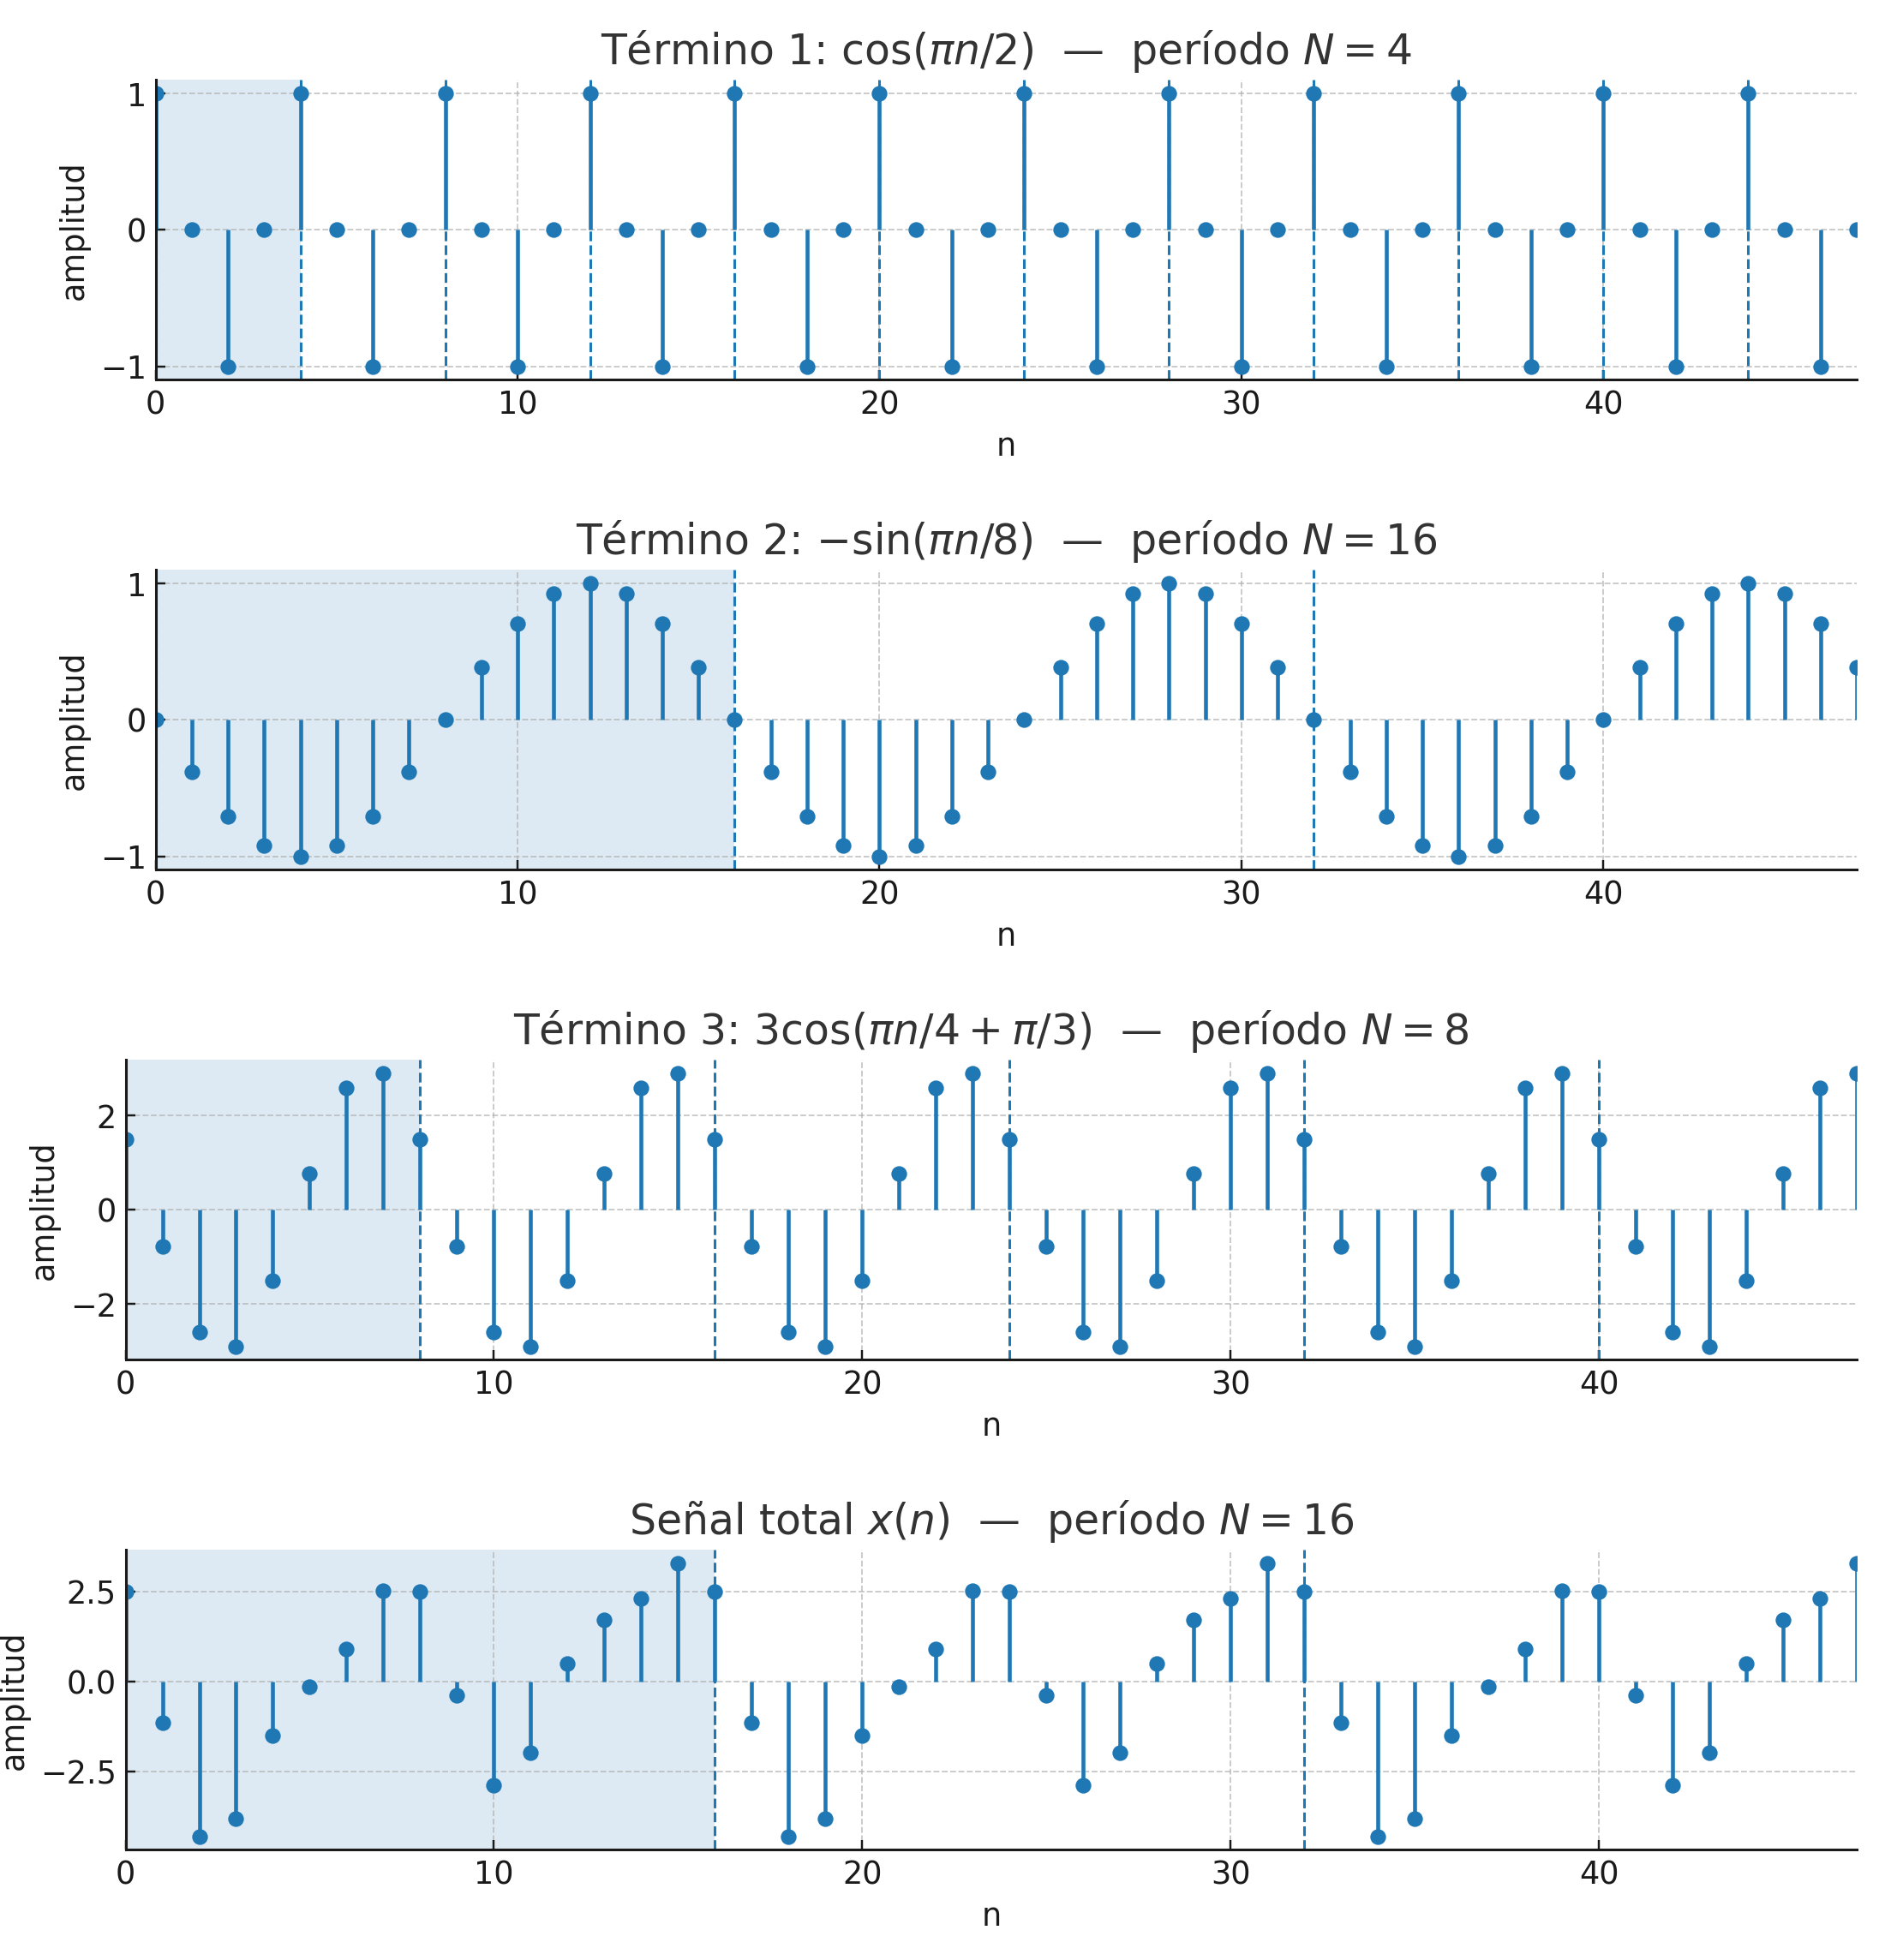
\includegraphics[width=0.5\textwidth]{Auxiliar_1_1}
            \caption{Diagrama de bloques}    
        \end{figure}
        \item Demuestre que los ceros de un sensor o filtro afectan la estabilidad del sistema. Puede utilizar el sistema anterior para plantear su desarrollo:
        \item emuestre que para un sistema SISO, los ceros de lazo cerrado son iguales a los ceros que se encuentran en lazo directo (ceros de lazo abierto) más los polos que se encuentran
        en el lazo de retroalimentación.
    \end{enumerate}
    %%%%%%%%%%%%%%%%%%%%%%%%%%%
    \begin{solution}
        \subsection*{Resolución 1.1}
        En primera instancia, se debe reconocer que la función de transferencia de cualquier sistema de control está dada por la razón entre la salida y la entrada del mismo. En este caso, la función que se debe encontrar debe relacionar la salida y la entrada de la forma $\frac{C(s)}{R(s)}$.A partir del diagrama de bloques se puede plantear el siguiente sistema de ecuaciones:
        \begin{align}
            E(s)&=R(s)-B(s) \label{eq:1} \\ 
            C(s)&=E(s)G(s) \label{eq:2} \\
            B(s)&=C(s)H(s) \label{eq:3}
        \end{align}
        Reemplazando (\ref{eq:1}) y (\ref{eq:3}) en (\ref{eq:2}) podemos desarrollar lo siguiente:
        \begin{align}
            C(s)&=(R(s)-B(s))G(s) \nonumber \\
            C(s)&=(R(s)-C(s)H(s))G(s) \nonumber \\
            C(s)&=R(s)G(s)-C(s)H(s)G(s) \nonumber \\
            C(s)+C(s)H(s)G(s)&=R(s)G(s) \nonumber \\
            C(s)(1+G(s)H(s))&=R(s)G(s) \nonumber \\
            \frac{C(s)}{R(s)}&=\frac{G(s)}{1+G(s)H(s)} \label{eq:final} 
        \end{align}
        
        Finalmente, la función de transferencia equivalente del diagrama está dada por la expresión (\ref{eq:final})
\subsection*{Resolucion 1.2}
Tal como se dijo en la clase auxiliar, las funciones de transferencia se pueden expresar como una división de polinomios en el dominio de Laplace. Por lo tanto, una función de trasnferencia $X(s)$ arbitraria se puede expresar según (\ref{eq:b})
\begin{equation}
    X(s)=\frac{s^m+\alpha_{m-1} s^{m-1}+...+\alpha_0}{s^n + \beta_{n-1}s^{n-1}+...+\beta_0} \quad m\leq n \label{eq:b}
\end{equation}

Notar que las funciones de transferencia nunca pueden ser \textbf{IMPROPIAS}, puesto que al descomponer su respuesta en el dominio del tiempo nos resulta un sistema físico que no representa una situación real. Por lo tanto, cuando en un futuro diseñen constroladores, siempre verifiquen que la función de transferencia sea \textbf{PROPIA} ($m\leq n$) o \textbf{BIPROPIA} ($n=m$).\\

Ahora bien, considerando lo descrito en (\ref{eq:b}), nosotros podemos generalizar los polinomios del numerador y del denominador. Lo anterior lo hacemos utilizando la definición de polos y ceros. Los polos son las raíces del denominador, por lo que multiplicando las raíces podemos recuperar el polinomio original. Esto se puede realizar de manera análoga para el numerador. De esta forma, las funciones $G(s)$ y $H(s)$ se pueden expresar de la siguiente forma:
\begin{align}
    G(s)&=\frac{\Pi (s+z^{G})}{\Pi (s+p^{G})} \label{eq:g} \\
    H(s)&=\frac{\Pi (s+z^{H})}{\Pi (s+p^{H})} \label{eq:p}
\end{align}
Para poder demostrar lo que se pide, debemos probar que los ceros de la función $H(s)$ aparecen de alguna forma en los polos de la expresión a lazo cerrado del sistema. Esto se debe a que, para probar que "algo" influye en la estabilidad, la mayoría de las veces se analizan las raíces de la ecuación característica $1+G(s)H(s)$ (que es justamente el denominador de la expresión (\ref{eq:final})). Por lo tanto, basta con reemplazar las ecuaciones (\ref{eq:g}) y (\ref{eq:p}) en (\ref{eq:final}):
\begin{align}
    \frac{C(s)}{R(s)} &= \frac{\frac{\prod (s+z^{G})}{\prod (s+p^{G})}}{1 + \frac{\prod (s+z^{G})}{\prod (s+p^{G})}\frac{\prod (s+z^{H})}{\prod (s+p^{H})}} \nonumber \\
    &= \frac{\prod (s+z^{G}) \prod (s+p^{H})}{\prod (s+p^{G}) + \prod (s+z^{G}) \prod (s+z^{H})} \label{eq:b_final}
\end{align}
De la expresión (\ref{eq:b_final}) se puede ver que en el denominador se encuentran los términos asociados a los ceros del sensor $(s+z^H)$. Por lo tanto, dado que los ceros aparecen en el denominador, estos afectan a la ecuación caraterística y por ende a la estabilidad.

\subsection*{Resolucion 1.3}
Para responder esta pregunta, basta notar la expresión descrita en (\ref{eq:b_final}). De esta ecuación se puede observar que su numerador está compuesto por los términos $\Pi (s+z^{G}) \Pi (s+p^{H})$, los cuales corresponden a los ceros de la función $G(s)$ y a los polos de la función $H(s)$. Dado que en el numerador de la función de lazo cerrado se encuentran los polos de lazo cerrado, entonces queda demostrado lo que se pide.
    \end{solution}
    %%%%%%%%%%%%%%%%%%%%%%%%%%%
    \question Encuentre el LGR del siguiente sistema:
    \begin{figure}[h!]
        \centering
        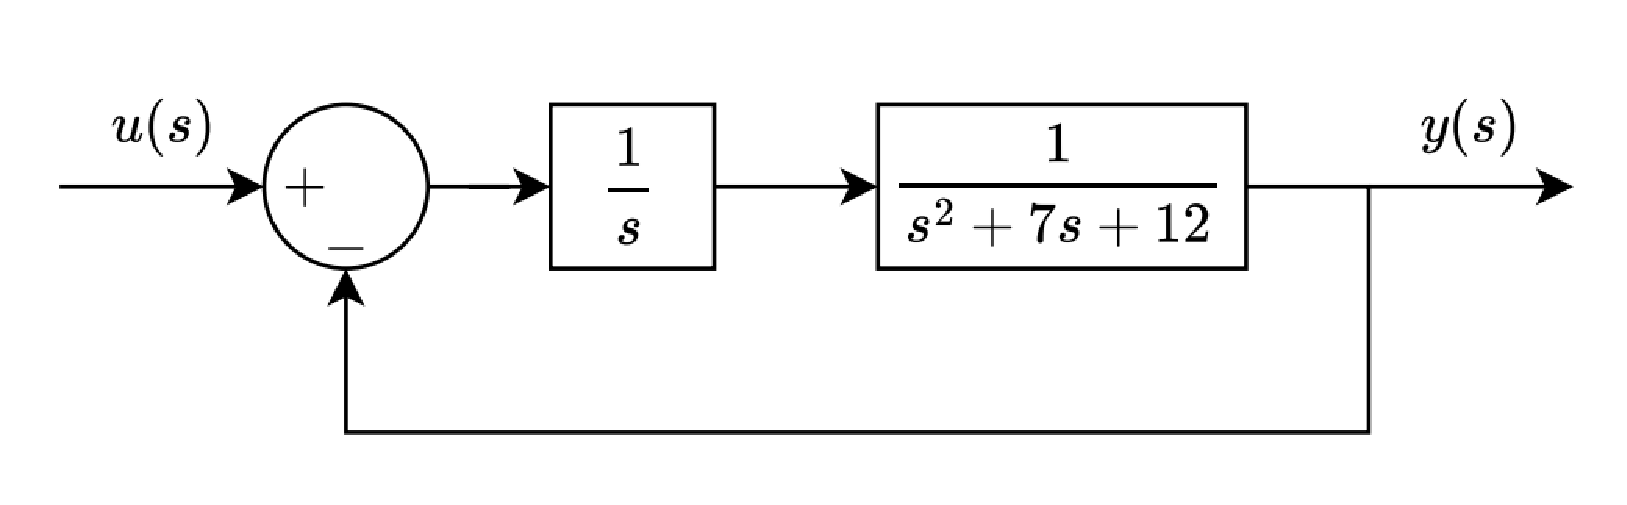
\includegraphics[width=0.5\textwidth]{Auxiliar_1_2}
    \end{figure}
    \begin{enumerate}
        \item ¿Es posible saber cuántos polos de lazo cerrado hay sólo mirando el LGR?
        \item ¿Es posible saber dónde estarán ubicados los polos de lazo cerrado?
        \item ¿Cuáles son los polos dominantes del sistema?
    \end{enumerate}
%%%%%%%%%%%%%%%%%%%%%%%%%%%
\begin{solution}
\subsection*{Resolucion 2.1}
    Se busca obtener el lugar geometrico de la raiz (LGR), por lo que se debera tener varios aspectos en cuenta.En primera instancia, se debe reconocer que el LGR es una representación gráfica de la variación de los polos de lazo cerrado a medida que se varía un parámetro del sistema. En este caso, el parámetro que se varía es el valor de $K$ asociado a la ganancia (Esto es equivalente a un controlador proporcional que veremos mas adelante, por ahora se puede entender como un parametro que podemos variar para que los polos se muevan a lo largo del LGR). De la primera pregunta obtuvimos que la funcion de transferencia vendra dada por:
    \begin{align}
        \frac{C(s)}{R(s) }&= \frac{G(s)}{1+G(s)H(s)}
    \end{align} 
    Donde G(s) corresponde a la pondearcion de todos los elementos del lazo directo, es decir que si existira un controlador $G_{c}$ y la planta $G_{p}$, luego $G(s) = G_{c} \cdot G_{p}$ , esto se obtiene directamente del desarrollo de bloques. Debemos recordar que la funcion de transferencia es una propiedad propia del sistema que dependera de variables de estados y no de las entradas (Recordartorio de su curso de Dinamicos). Se debe tener un gran cuidado entre la la diferencia de los polos de lazo abierto ($G(s) \cdot H(s)$) y de lazo cerrado ($1+G(s) \cdot H(s)$),debido a que este ultimo da cuenta del lazo de retroalimentacion.Como se menciono anteriormente el LGR nos entrega una representacion visual del movimiento de los polos \textbf{de lazo cerrado} de la funcion de transferencia vista anteriromente. Por lo tanto tendremos que esos polos deberan cumplir que:
    \begin{align}
        1+G(s)H(s) &= 0\\
        G(s)H(s) &= -1
    \end{align}
    Por lo que para que se cumpla dicha condicion se deben cumplir dos criterios
    \begin{itemize}
        \item \textbf{Condicion de modulo:} Se debe cumplir que $|G(s)H(s)| = 1$ 
        \item \textbf{Condicion de angulo:} Se debe cumplir que $\angle G(s)H(s) = \pm 180^{\circ} + n360^{\circ}$ 
    \end{itemize}
Por lo que todos los puntos $s = \sigma + j\theta$ que cumplan ambas condiciones perteneceran al LGR y seran los polos de lazo cerrados de su sistema. Comenzamos identificando los polos y ceros de la funcion de transferencia de lazo abierto (Que representaran nuestros puntos de partida) , dados por :
\begin{align}
    G(s)H(S)= \frac{1}{s} \frac{(s+2)}{(s^{2} +7s +12)} = \frac{1}{s} \frac{(s+2)}{(s+3)(s+4)}
\end{align}
(Consideramos que $H(s)=1$, dado que no tenemos informacion de esta funcion de transferencia), con lo que identificamos que los polos de lazo abierto son $p_1=0$ , $p_2=-3$ y $p_3=-4$ y los ceros son $z_1=-2$. Por lo que se posiciona en el LGR
\begin{center}
    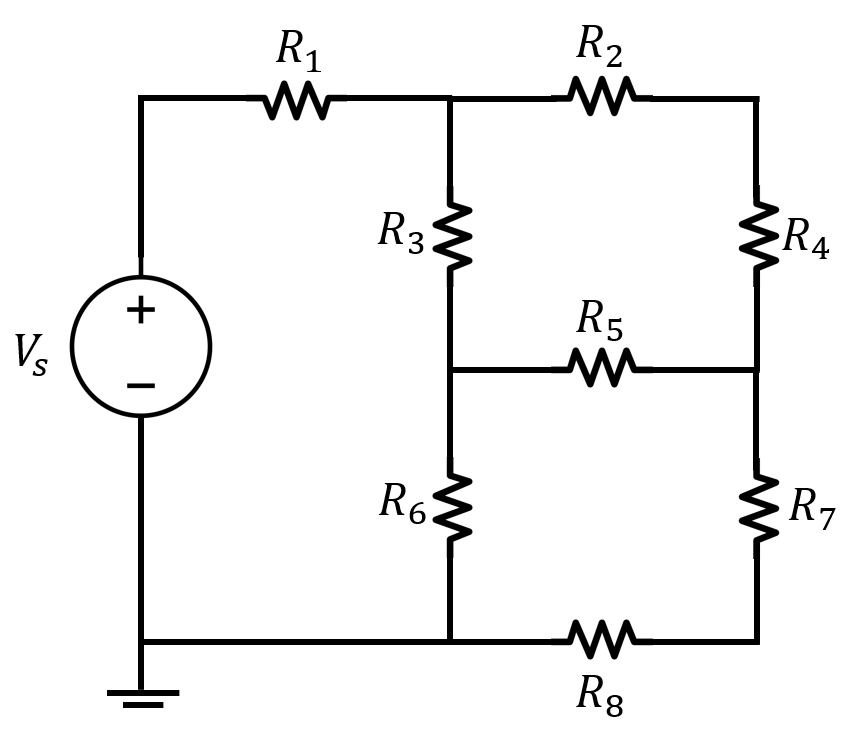
\includegraphics[width=0.65\textwidth]{Auxiliar_1_3}
    \captionof{figure}{LGR ubicacion de los polos}
  \end{center}
Luego se debe encontrar las zonas en el eje real que pertenecen al LGR, esto se puede obtener de dos formas, una considerando la condicion de angulo, la cual se ejemplifica de buena manera en lo siguiente
\begin{center}
    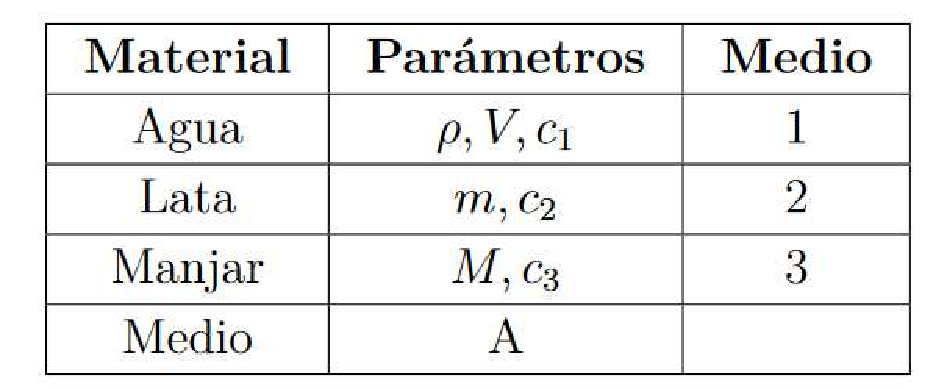
\includegraphics[width=0.65\textwidth]{Auxiliar_1_4}
    \captionof{figure}{Lugar donde no se cumple la condicion de angulo en el eje real}
\end{center}
\begin{center}
    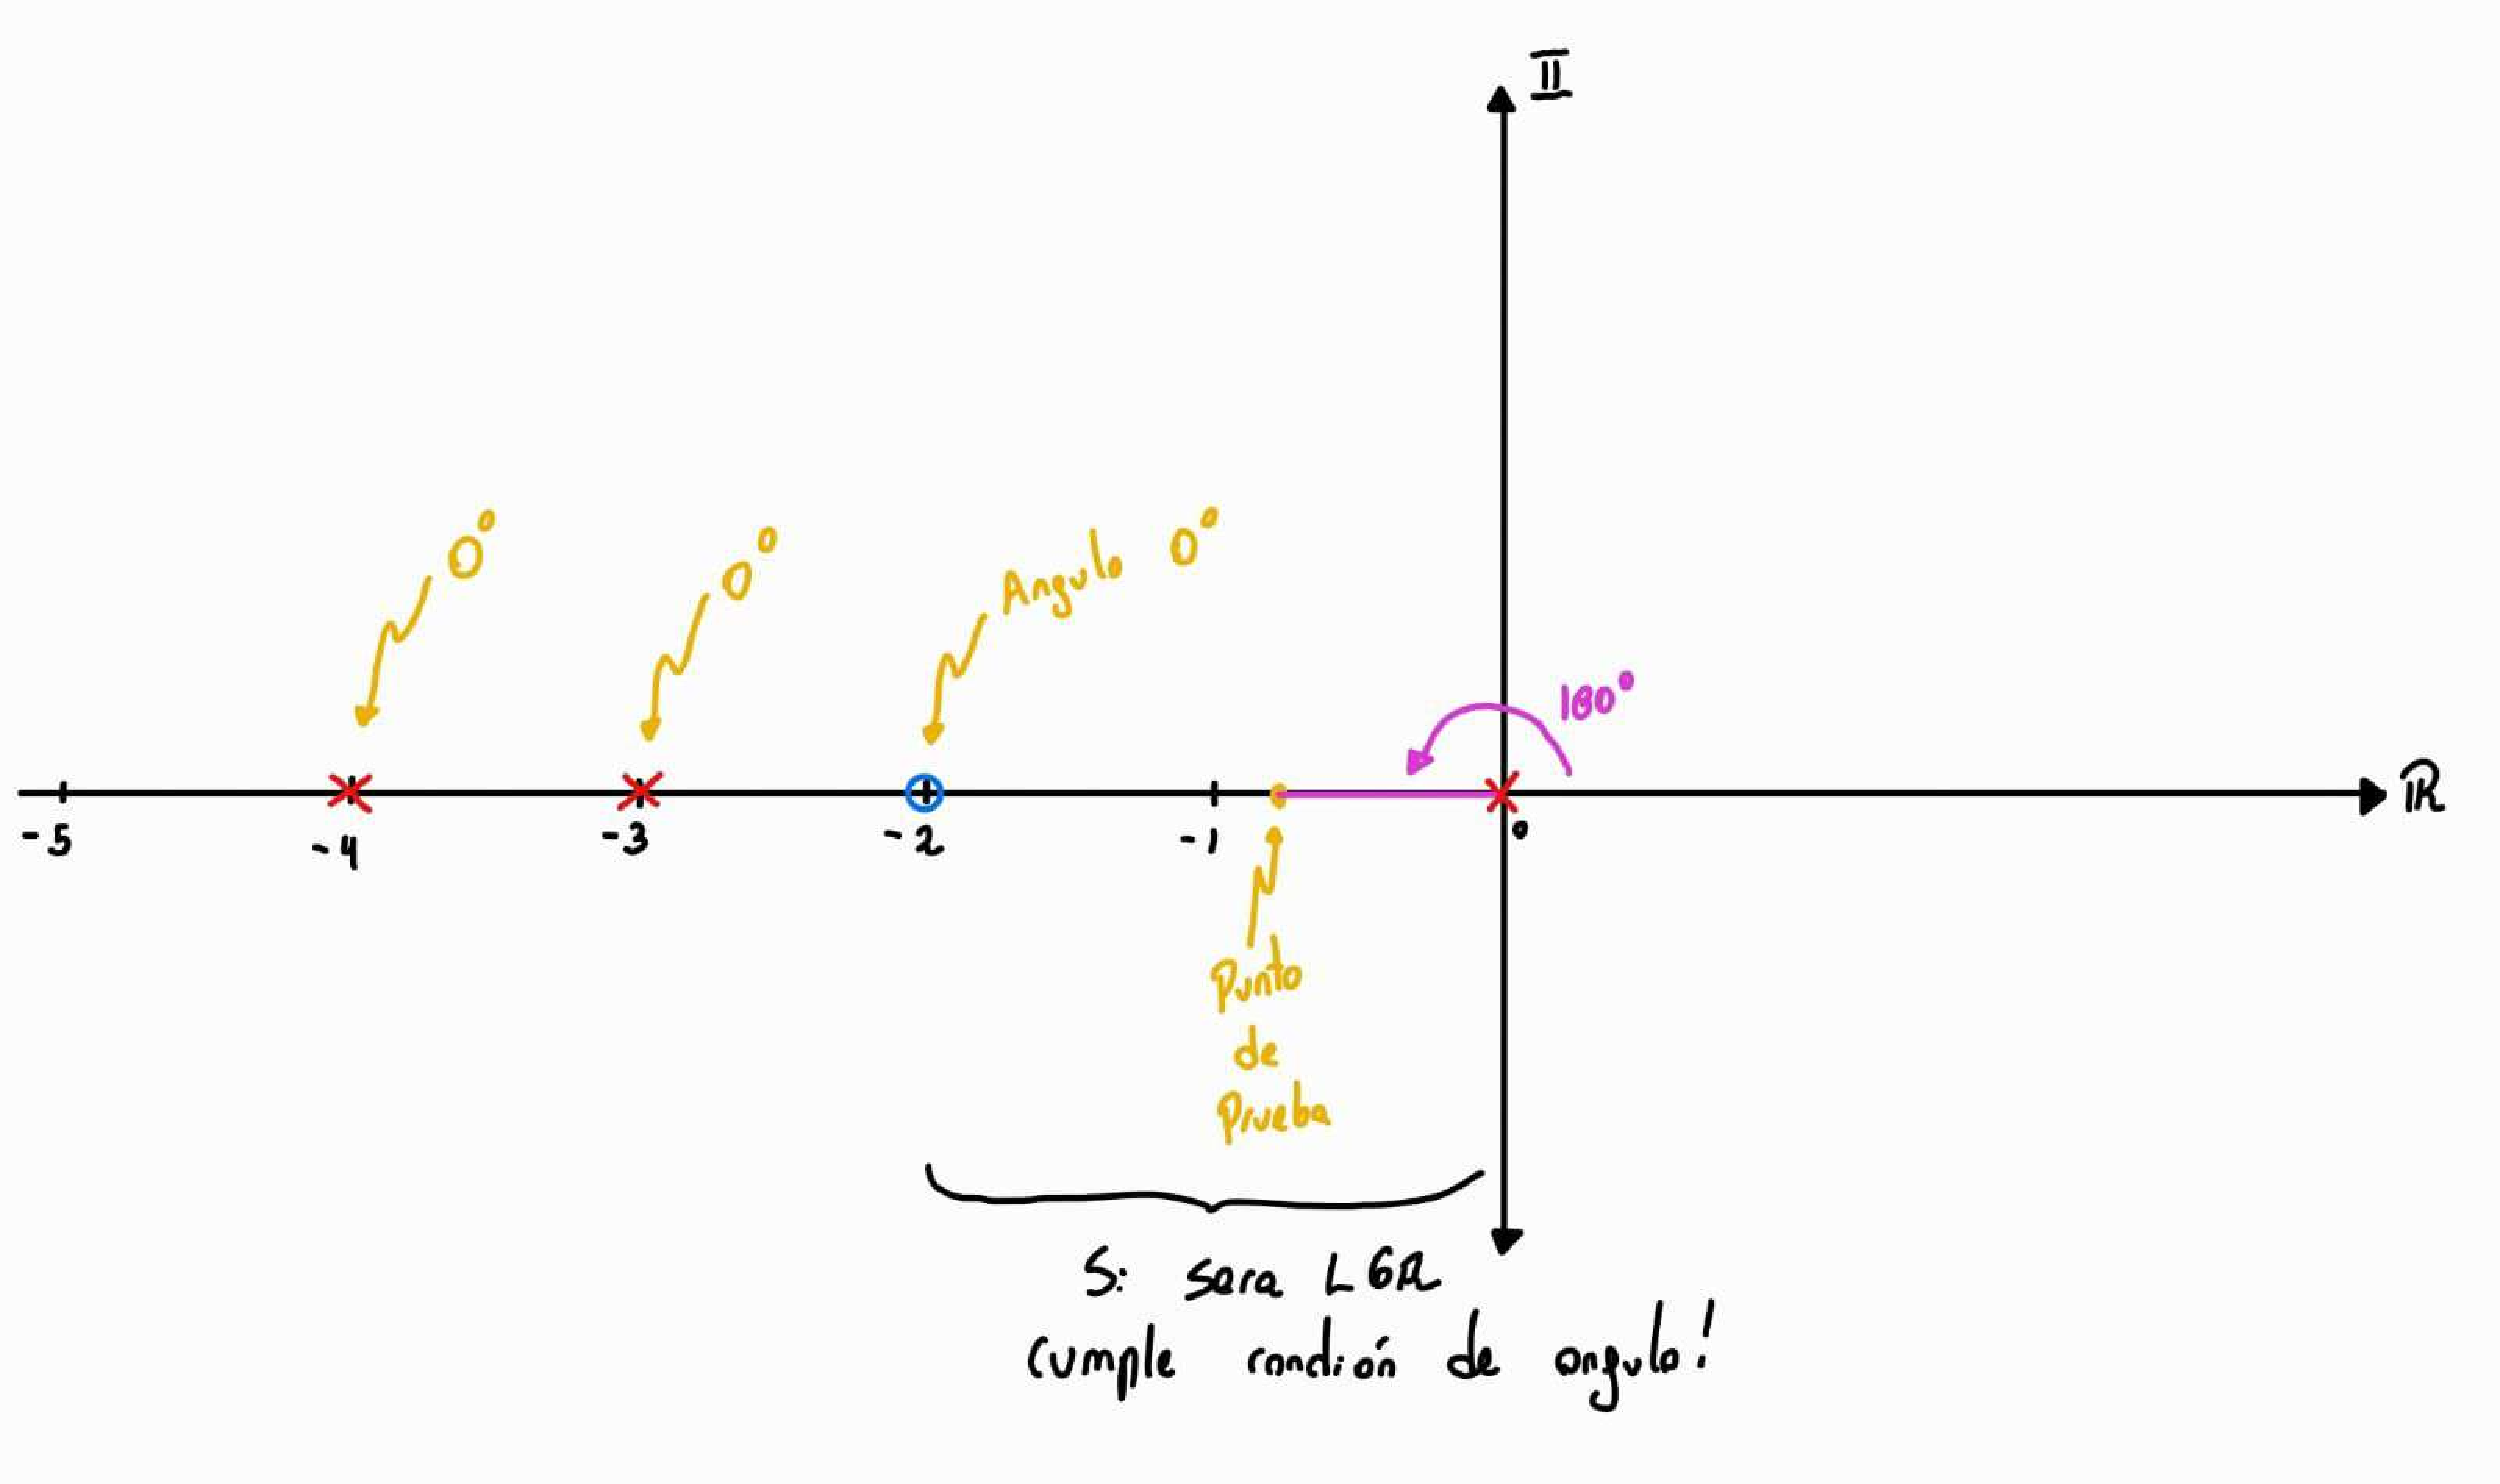
\includegraphics[width=0.65\textwidth]{Auxiliar_1_5}
    \captionof{figure}{Lugar donde se cumple la condicion de angulo en el eje real}
\end{center}
\begin{center}
    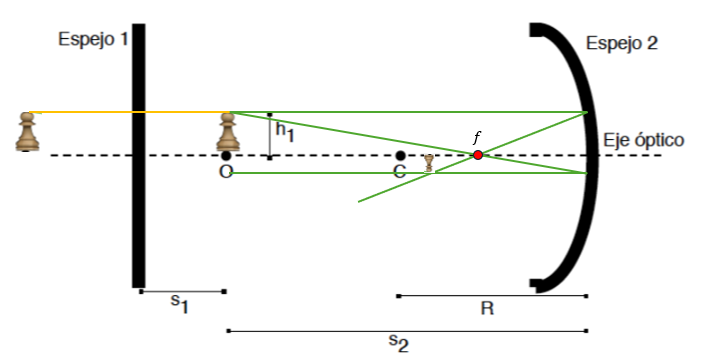
\includegraphics[width=0.65\textwidth]{Auxiliar_1_6}
    \captionof{figure}{LGR de la zona real}
  \end{center}
Otra forma (la que yo recomiendo de manera personal) es considerar la siguiente regla. En ambos casos me posiciono en un polo o un cero.
\begin{itemize}
    \item Si la cantidad de polos es \textbf{PAR} luego esa zona no pertenecera al LGR
    \item Si la cantidad de polos es \textbf{IMPAR} luego esa zona pertenecera al LGR
\end{itemize}
Es una forma rapida, y se puede verificar mediante la condicion de angulo. Una vez identificadas las zonas del LGR en la zona real, deberemos obtener el lugar de las asintotas la cual se define como:
\begin{align}
    \sigma = \frac{\sum polos - \sum Ceros}{ \# Asintotas = \# Polos - \# Ceros}
\end{align}
Con lo que en nuestro caso particular da como resultado a:
\begin{align}
    \sigma = \frac{(0-3-4 )-(-2)}{2} = -2.5
\end{align}
\begin{center}
    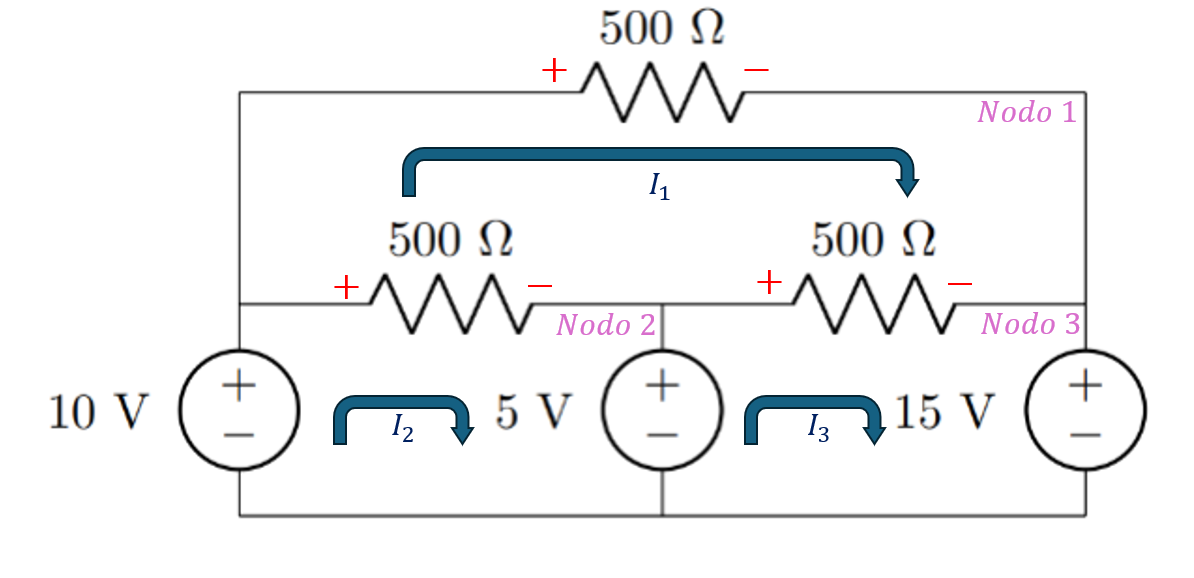
\includegraphics[width=0.65\textwidth]{Auxiliar_1_7}
    \captionof{figure}{Lugar de ubicacion de la asintota }
  \end{center}
Una vez se obtiene la posicion de las asintotas se debera obtener los angulos asociados a esta, las cuales vienen dadas por (\textbf{SOLO PARA GANANCIA POSITIVA $K>0$}):
\begin{align}
    \Theta_{k} = \frac{(2k+1)\pi}{\#asintotas}
\end{align}
Donde el dominio de $k \in \{0,...,\#Asintotas -1 \}$ , por lo que en nuestro caso correspondera a:
\begin{align}
    \Theta_{0} = \frac{\pi}{2} = 90^{\circ} \quad \Theta_{1} = \frac{3\pi}{2}= 270^{\circ}
\end{align}
Por lo que al ser graficadas se obtiene el siguiente esquema:
\begin{center}
    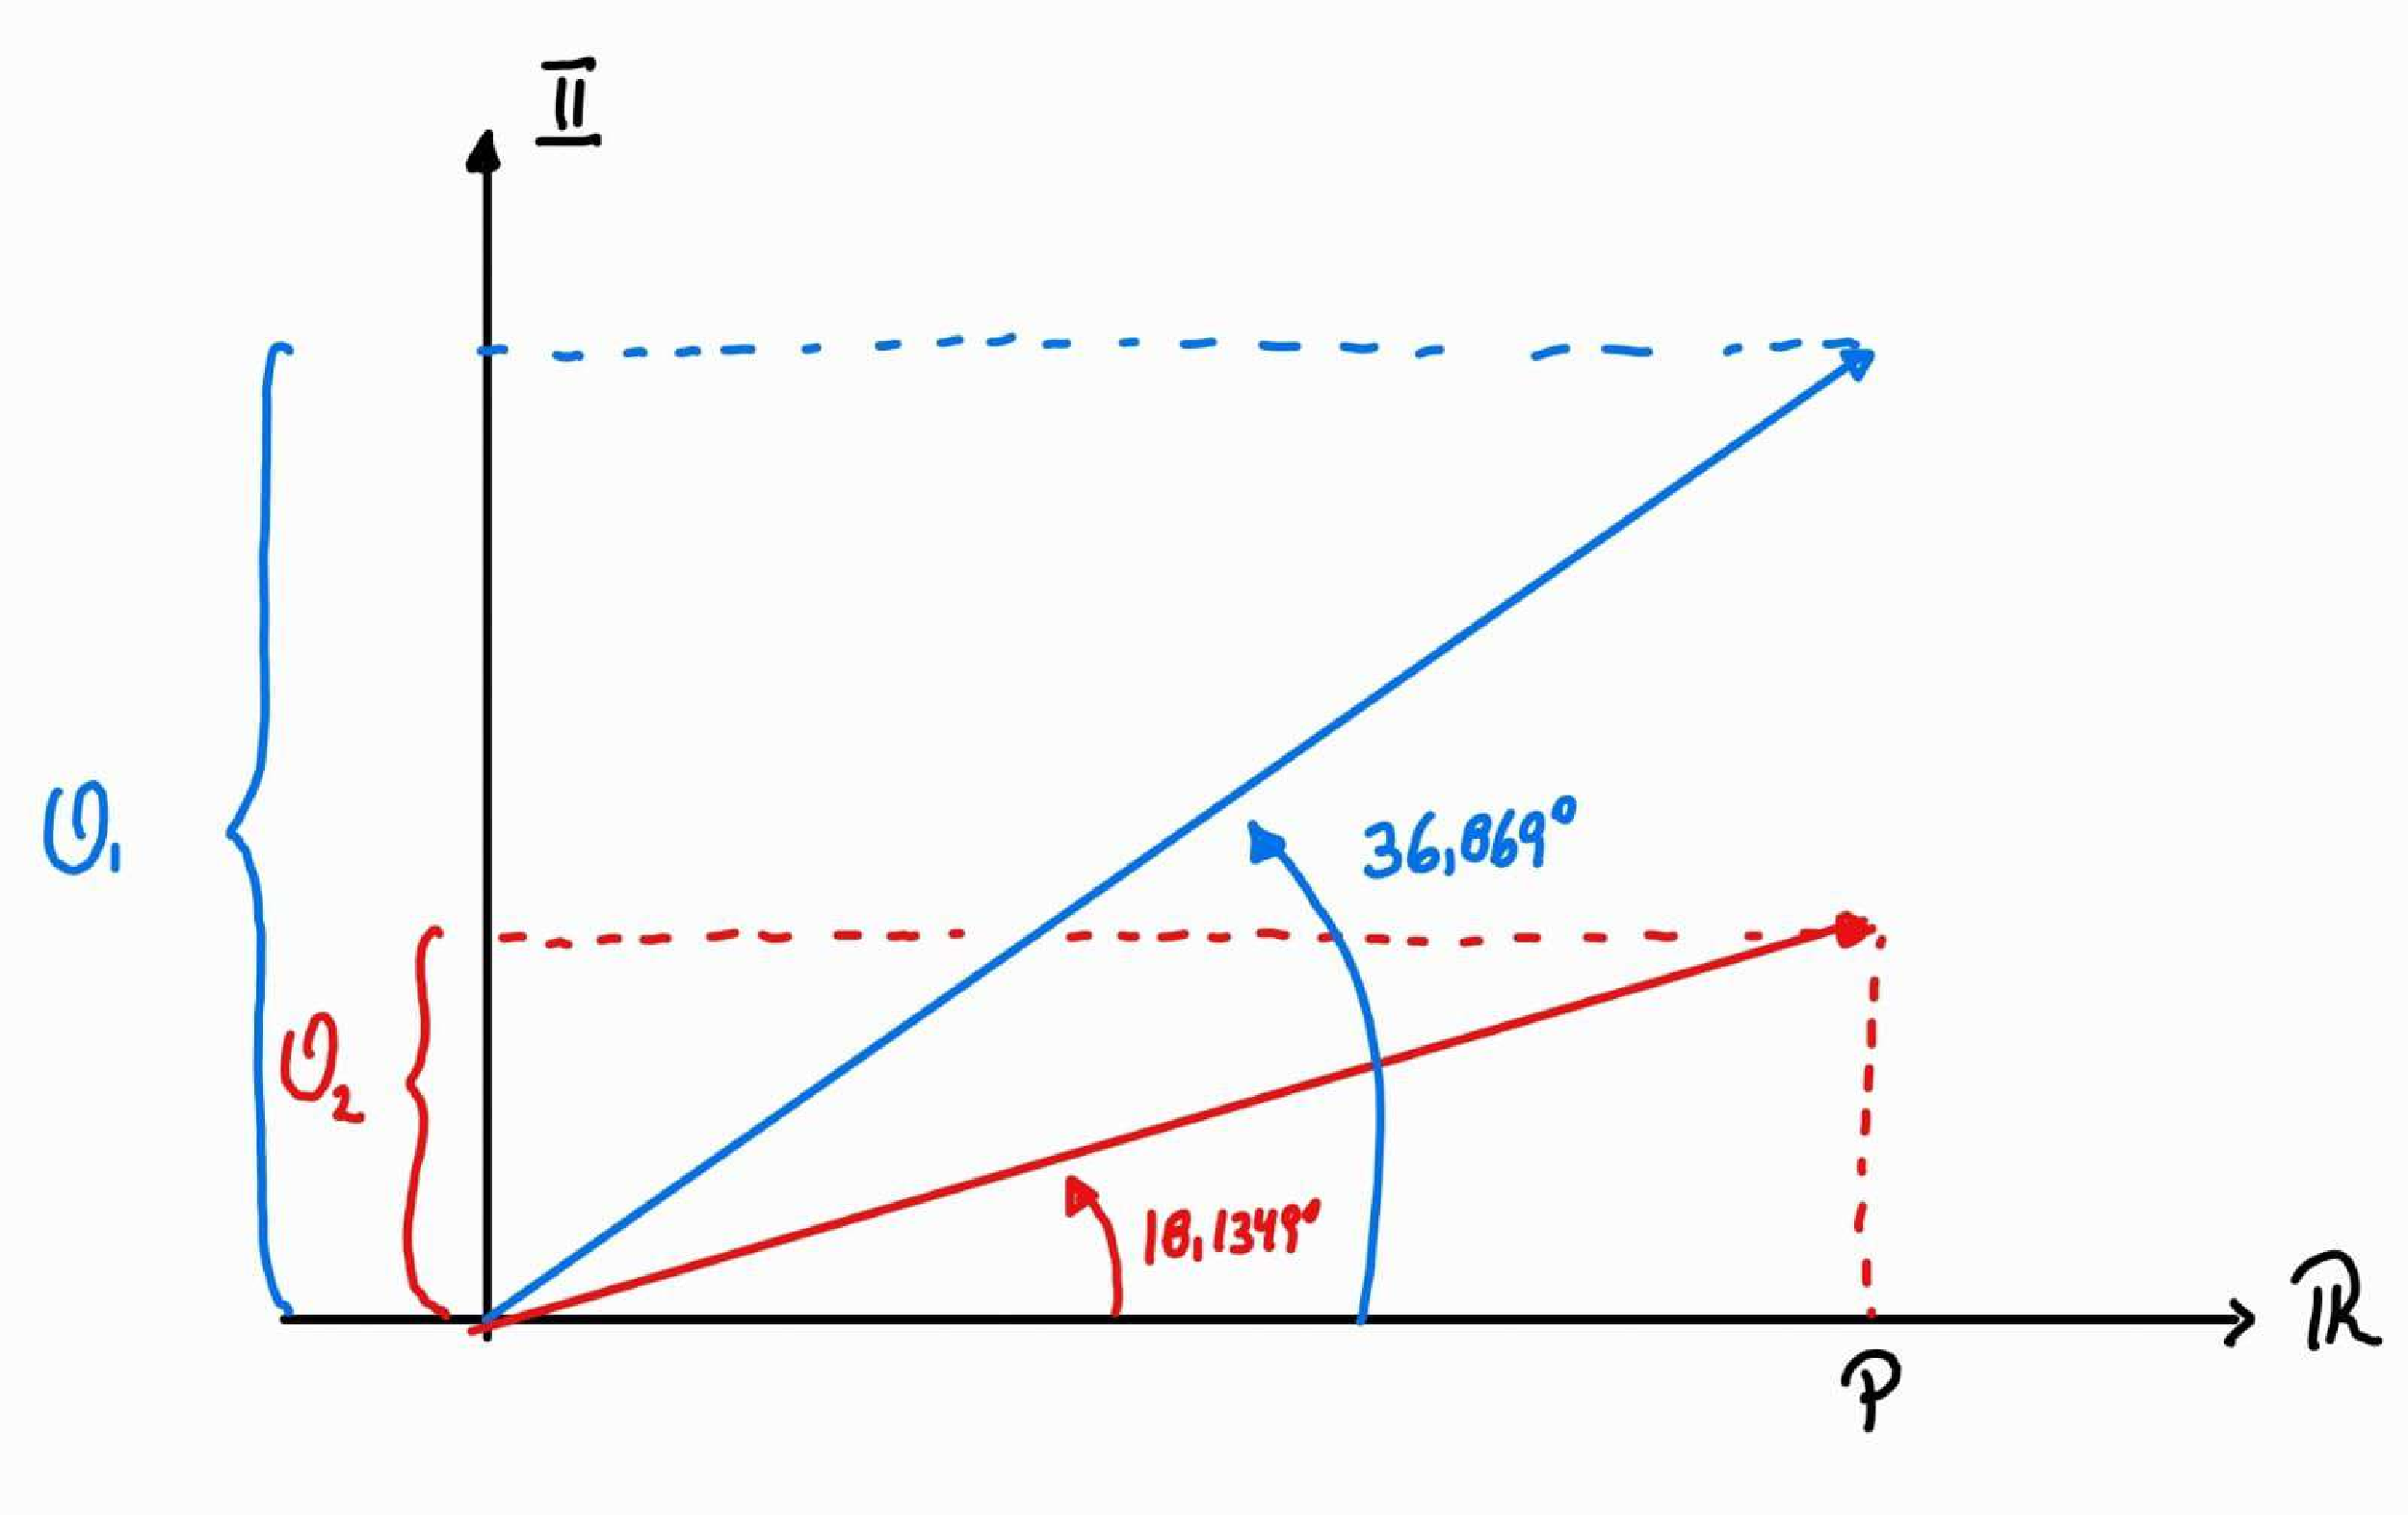
\includegraphics[width=0.65\textwidth]{Auxiliar_1_8}
    \captionof{figure}{Angulos relacionados a las asintotas }
  \end{center}
Por ultimo deberemos obtener el punto de llegada o salida que tiene relacion con los donde los polos de lazo cerrado divergen en el plano complejo o donde llegan. Esto se obtiene de la siguiente manera:
\begin{align}
    1+kG(s)H(s) &= 0\\
    1+k\frac{1}{s} \frac{(s+2)}{(s+3)(s+4)} &= 0\\
    k & = -\frac{s(s+3)(s+4)}{s+2}
\end{align}
Luego esta expresion se deriva e iguala a 0 (\textbf{Recomiendo ver el apunte del profe donde se entiende mas la idea}), una breve intuicion de lo que sucede, viene dado por el hecho de que encontramos el $\sigma$ (parte real) maxima o minima de s , antes de que esta pase a ser compleja, y deje el plano real, de esta manera se obtiene que:
\begin{align}
    \frac{\partial K}{\partial s} &= \frac{(3s^{2} +14s+12)(s+2) + (s^{3} + 7s^{2} +12s)}{(s+2)^{2}} = 0\\
    &=-2s^{3}-13s^{2}-28s-24=0
\end{align}
Dando como resultados los siguientes polos:
\begin{align}
    s_{1} &= -3.43\\
    s_{2,3}&= -1.21\pm j1.073 
\end{align}
Notamos que estamos viendo valores de $s=\sigma$ es decir que deberan cumplir dos condiciones
\begin{enumerate}
    \item Debera pertenecer al LGR de la parte real
    \item Debera ser real dado que sobre esto se realiza el analisis
\end{enumerate}
De esta manera vemos que el unico punto que cumple dicha condicion corresponde a $s_{1}$, pueden darse situaciones en que no existan puntos de llegada o salida y sigue siendo valida, simplemente nos da a entender que no cruza el eje real, luego al añadirlo al frafico previo tenemos que:
\begin{center}
    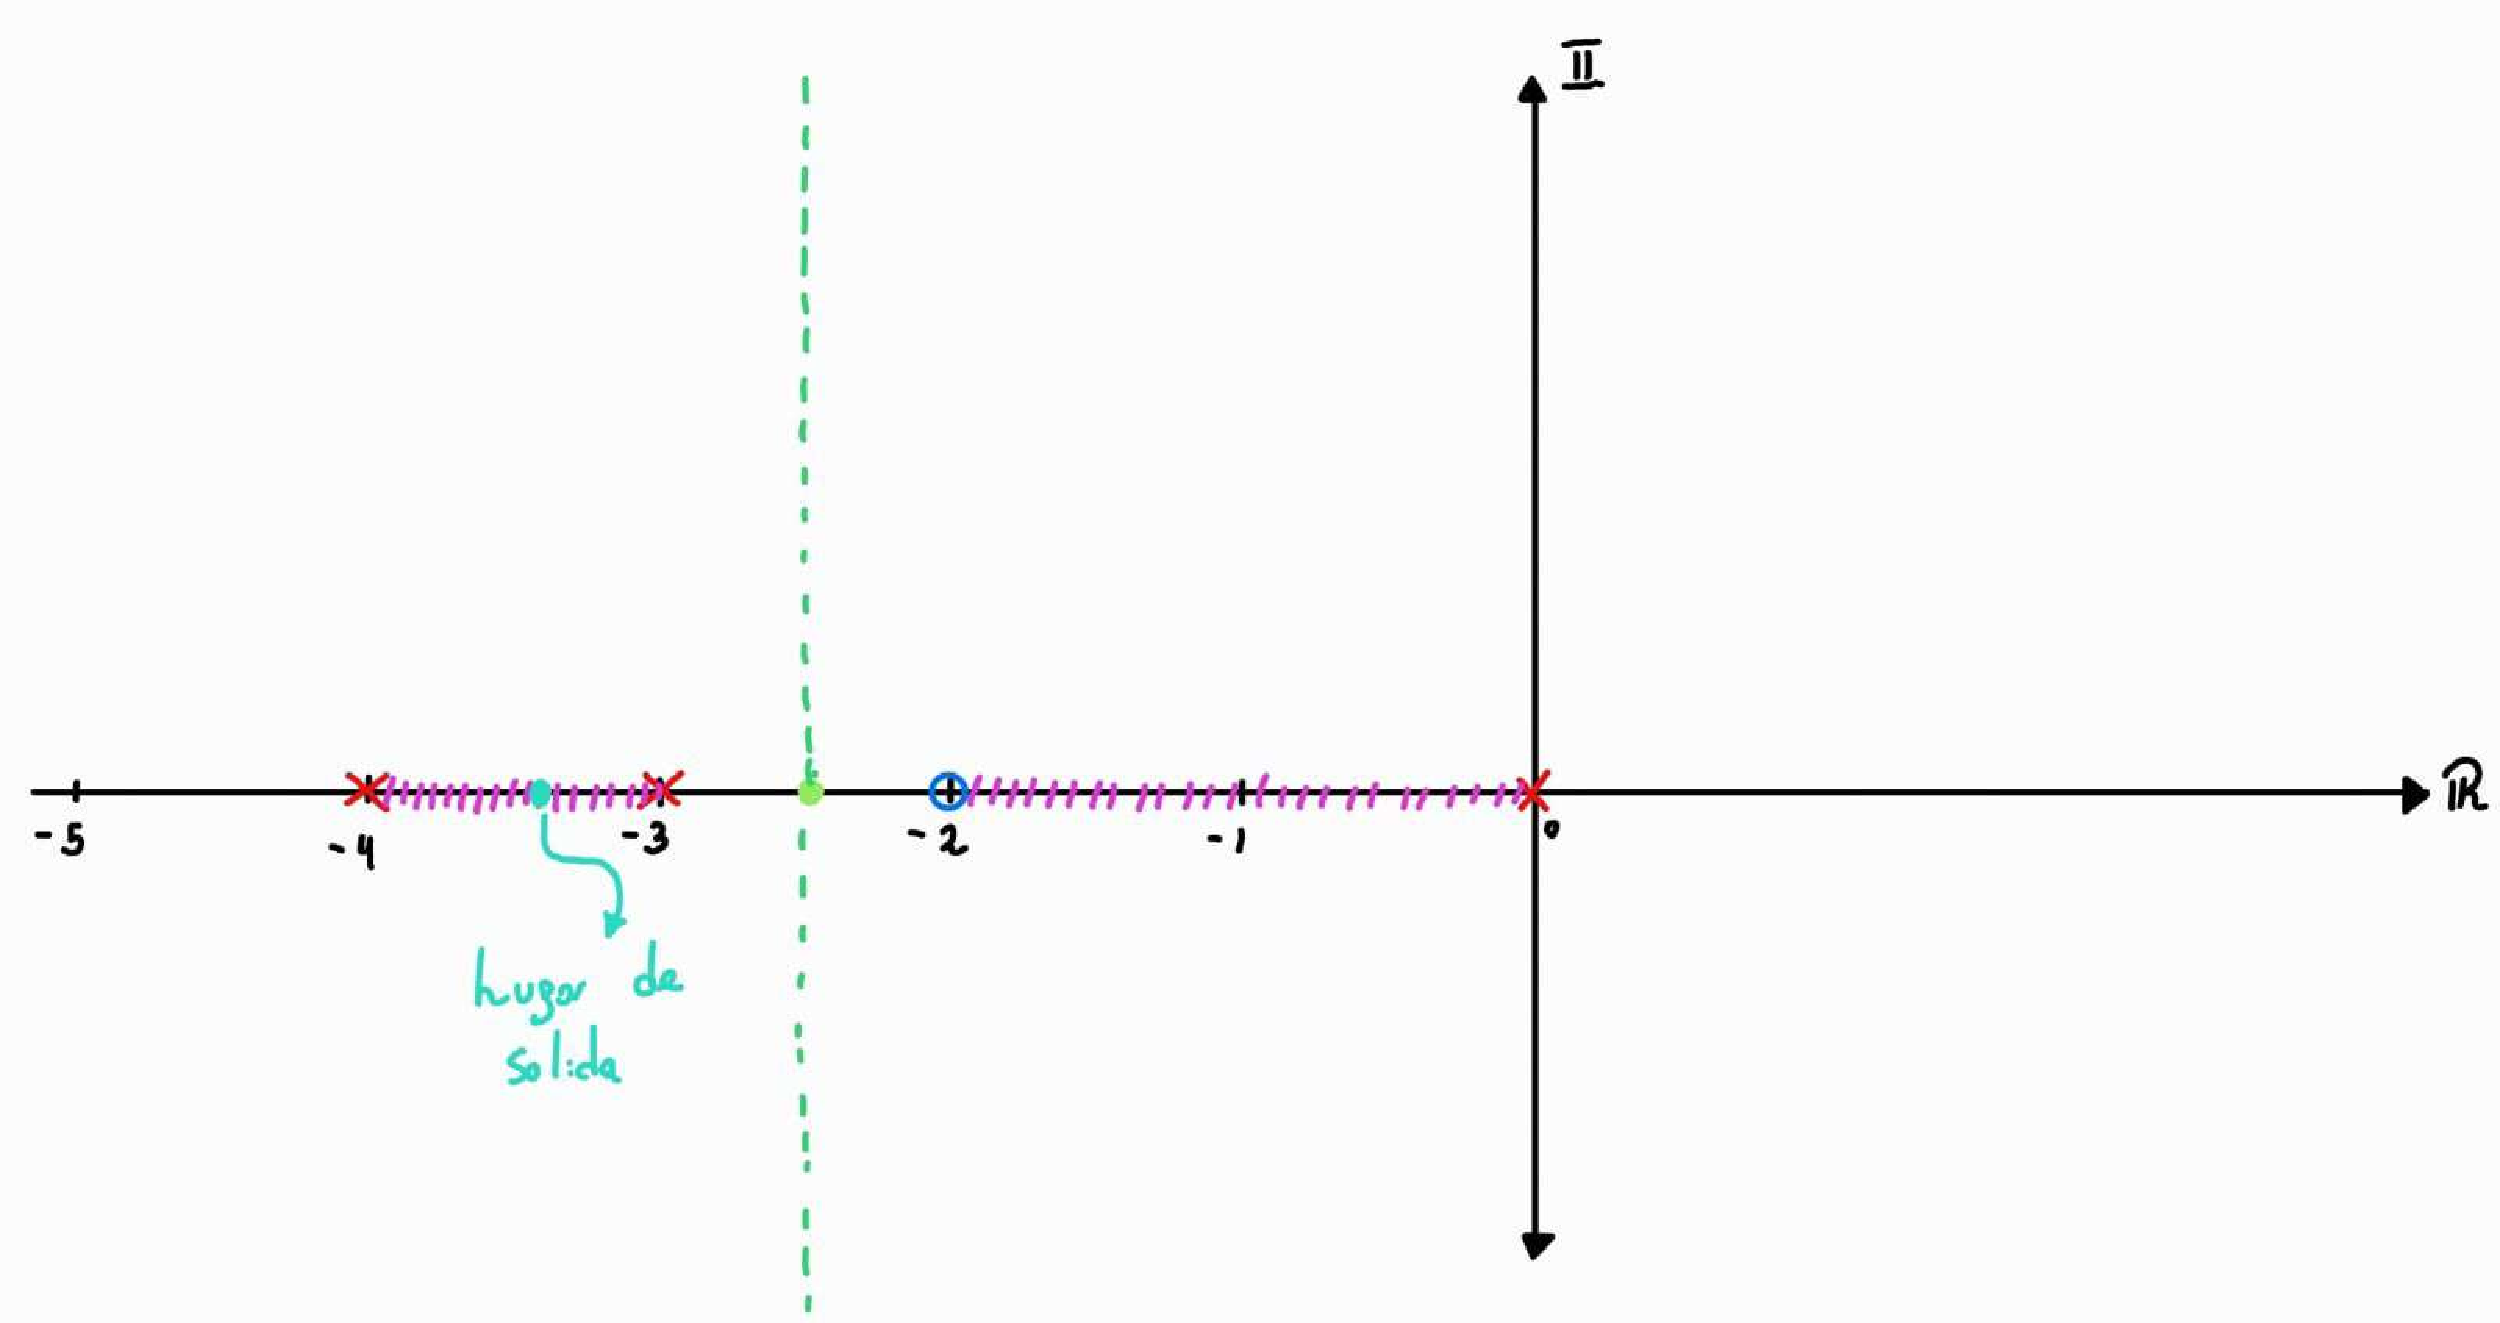
\includegraphics[width=0.65\textwidth]{Auxiliar_1_9}
    \captionof{figure}{Ubicacion del lugar de salida o llegada }
  \end{center}
Finalmente podemos graficar los polos de lazo cerrado, los cuales se encuentran en la siguiente imagen:
\begin{center}
    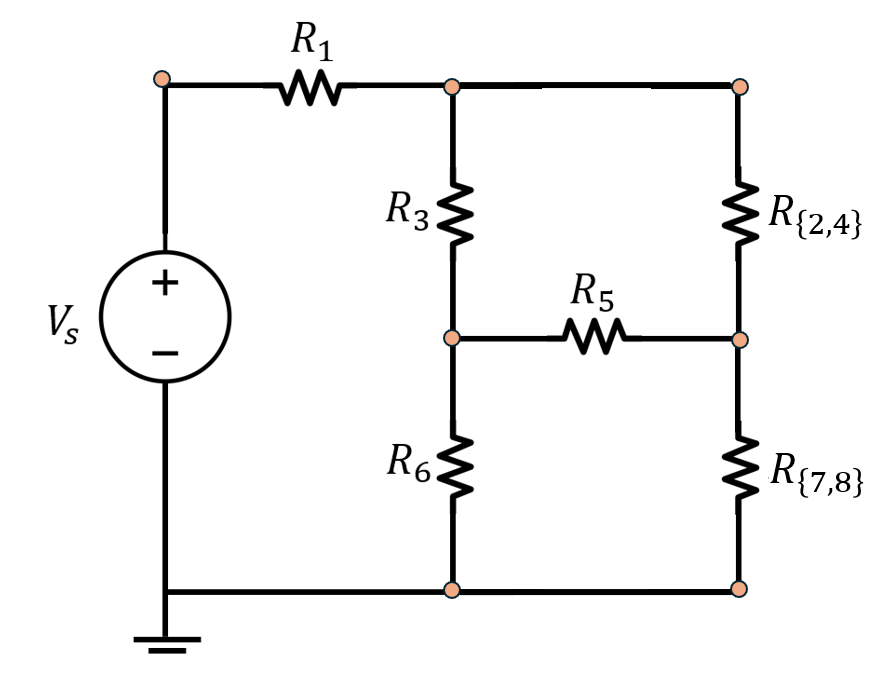
\includegraphics[width=0.65\textwidth]{Auxiliar_1_10}
    \captionof{figure}{LGR de polos de lazo cerado}
  \end{center}
Notamos que las lineas deben ser suaves y ademas debe ser simetrico con respecto al eje real, dado que los polos de lazo cerrado si son complejos estos deben ser conjugados, ademas la curva debe ser suave ,es decir no rectas. Una idea intuitiva para poder graficar el LGR esque los polos siempre iran a los ceros (Esto dado que para un k infinito convergen a ceros) y en caso de no existir mas ceros, los polos restantes divergen a las asintotas. Con lo que finalmente se responden las preguntas.
\begin{enumerate}
    \item Si , es posible dado que la cantidad de polos de lazo cerrado correspondera a la cantidad de polos de lazo abierto (Puntos de partida)
    \item Si es posible obtenerlo, mediante el LGR es la herramienta visual que nos permite obtener los polos de lazo cerrado para analizar estabilidad.
    \item Recordemos que los polos vienen del dominio del laplace , que en el dominio del tiempo corresponde a expresiones del tipo $Ae^{-pt}$ donde tenemos que la funcion de transferencia en el dominio del tiempo sera la suma de todos estos polos de la forma vista anteriormente, en donde que el polo sea mucho mayor nos indica que esta decae mucho mas rapido y no afectara tan rapido la respuesta,  mientras que los polos cercanos al cero seran los que afecten mas a la respuesta porque decaen mas lentos y por tanto perduran mas en el tiempo
\end{enumerate}


\end{solution}

%%%%%%%%%%%%%%%%%%%%%%%%%%%

\end{questions}
\newpage
%%%%%%%%%%%%%%%%%%%%%%%%%%%

\end{document}